\documentclass[12pt]{article}

\usepackage[]{inputenc}
\usepackage{graphicx}

\begin{document}

\title{Supplementary material for "XXX Title"}
\author{Eric Bazin, Keurcien Luu, Michael G. B. Blum}

\maketitle

\begin{figure*}[t]
\begin{center}
\includegraphics[height=0.8\textheight]{figures/environmentaldata.eps}
\end{center}
\caption{Graphical representation of mean environmental value for environment 4 to 10. Equation determining the environment is given in the main manuscript. Mean environmental value for environment 4, 5 and 6 are respectively equivalent to environment 1, 2 and 3.}%
\label{fig:simulatedenvir}%
\end{figure*}

\begin{figure*}[t]
\begin{center}
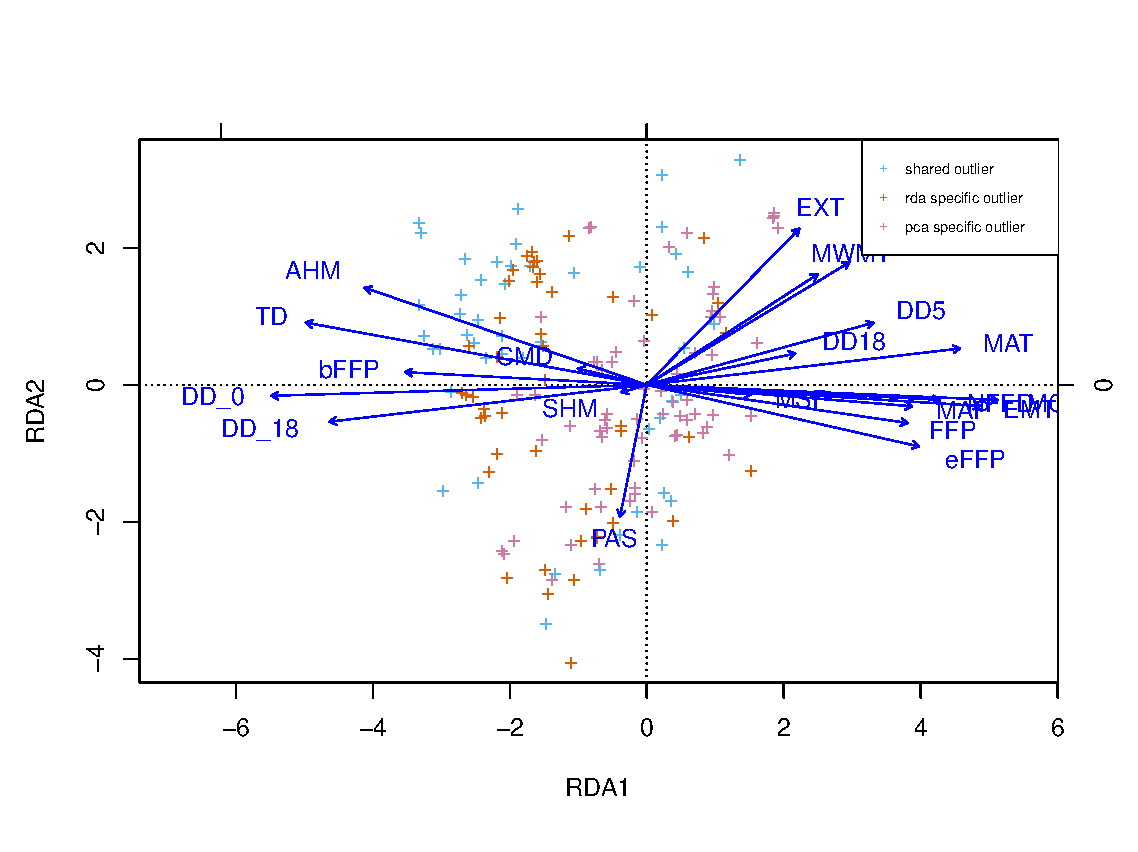
\includegraphics[height=0.6\textheight]{figures/poplar_rda.eps}
\end{center}
\caption{RDA analysis on \textit{Poplar trichocarpa} adaptive enriched genetic space. The first two axis RDA1 and RDA2 explain 37.8 and 14.0\% of variance predicted by environmental variable (22.7\% of constrained variance). Specific and shared outliers between PCA based method and RDA based method are differentially colored.}%
\label{fig:poplarrda}%
\end{figure*}

\begin{figure*}[t]
\begin{center}
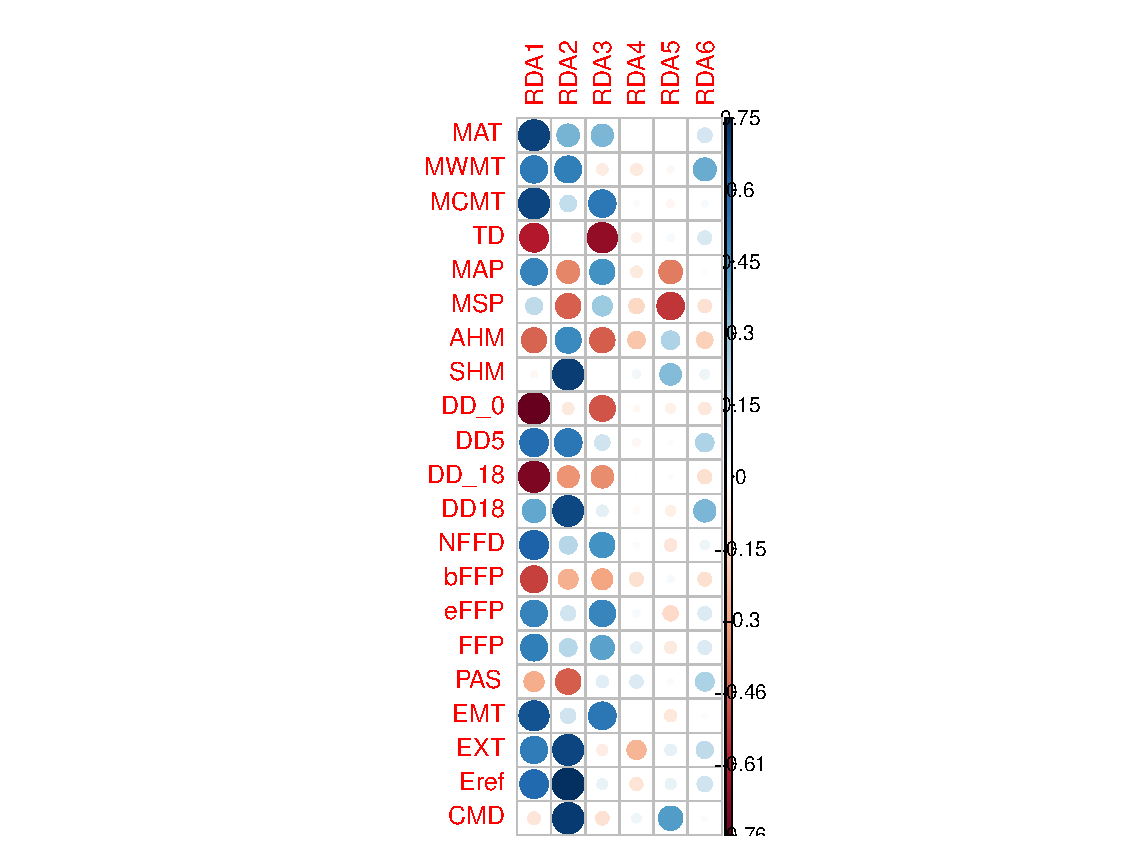
\includegraphics[height=0.6\textheight]{figures/corrplot.eps}
\end{center}
\caption{biplot of RDA analysis. Color and circle diameter are proportional to the amount of linkage between RDA axis and climatic variable.}%
\label{fig:corrplot}%
\end{figure*}



\end{document}
